\documentclass[11pt]{article}

\usepackage[margin=1in]{geometry}
\usepackage[colorlinks=true, linkcolor=blue, urlcolor=blue]{hyperref}
\usepackage{xurl}
\usepackage{enumitem}
\usepackage{longtable}
\usepackage{array}
\usepackage{xcolor}
\usepackage{titlesec}
\usepackage{booktabs}
\usepackage{tikz}
\usetikzlibrary{positioning, arrows.meta, shapes.geometric, fit, backgrounds, calc}

\definecolor{brand}{HTML}{1F4E79}
\definecolor{slow}{HTML}{8E44AD}
\definecolor{fast}{HTML}{C2185B}
\titleformat{\section}{\large\bfseries\color{brand}}{\thesection.}{0.6em}{}
\titleformat{\subsection}{\normalsize\bfseries\color{brand}}{}{0em}{}
\setlist[itemize]{leftmargin=1.4em, topsep=2pt}
\setlist[enumerate]{leftmargin=1.6em, topsep=2pt}

\newcommand{\code}[1]{\texttt{#1}}

% ---- shared TikZ styles -------------------------------------------------
\tikzset{
  proc/.style={draw=brand, rounded corners, fill=brand!8, align=center,
               text width=23mm, minimum height=11mm, font=\small},
  store/.style={cylinder, shape border rotate=90, aspect=0.28, draw=brand,
                fill=brand!18, align=center, text width=34mm, minimum height=16mm,
                font=\small\bfseries, inner sep=1mm},
  io/.style={draw=brand, rounded corners, fill=white, align=center,
             text width=23mm, minimum height=11mm, font=\small},
  dec/.style={draw=brand, diamond, aspect=2, fill=brand!8, align=center,
              text width=20mm, inner sep=0pt, font=\footnotesize},
  lane/.style={draw, thick, dashed, rounded corners=3mm, inner sep=5mm},
  ar/.style={-{Latex[length=2.4mm]}, thick, brand},
  arb/.style={{Latex[length=2.4mm]}-{Latex[length=2.4mm]}, thick, brand},
}

\title{\textbf{UdaanHer Saathi --- App Plan v2}\\
\large A voice mentor that assesses, then teaches rural women to \emph{earn} ---\\
with content grounded in real tutorials, generalized to any skill}
\author{Team: Aishi + mentor}
\date{}

\begin{document}
\maketitle

\begin{center}\itshape\small
Supersedes the fixed-curriculum content model of the original spec (\S9, \S11).
A plan-level rethink: record the switch in \code{docs/decisions.md} before building.
\end{center}

\tableofcontents

% =========================================================================
\section{Vision and principles}

A \textbf{voice mentor} for rural women that first works out what she already knows, then
teaches her --- in short, spoken, personalized lessons \emph{grounded in real tutorials, not
invented} --- how to \textbf{earn} from a vocational skill. Any skill. Nothing about a specific
trade is hardcoded.

\begin{enumerate}
  \item \textbf{Earning-first.} The goal is income, not a certificate. Every skill's path ends in
  \emph{make something sellable $\rightarrow$ price it $\rightarrow$ find customers}, not just technique.
  \item \textbf{Voice-first.} Voice is the interface. She never has to read or tap. Visuals ---
  a real video clip, or a generated diagram --- are \emph{optional aids} the mentor offers, never
  required to follow the lesson.
  \item \textbf{Generalized, not hardcoded.} No skill lives in code. The teaching engine is
  skill-agnostic; skills are data the system \emph{produces}. The popular rural skills are just the
  pre-seeded library, not a cage.
  \item \textbf{Grounded, not invented.} Content is distilled from \emph{real} YouTube tutorials
  (via transcript / STT-translate), so it is trustworthy for a livelihood, where wrong advice has
  real cost. The mentor synthesizes and narrates; it never hallucinates a curriculum, and it never
  produces videos.
\end{enumerate}

% =========================================================================
\section{System architecture: a two-speed design}

The governing constraint (\S6) is that YouTube search $+$ transcript fetch is quota-limited and too
slow for a live conversation. That single fact splits the app into two lanes --- which also cleanly
resolves ``generalized \emph{and} content-we-create.'' The \textbf{slow lane} sources and caches
grounded material offline; the \textbf{fast lane} assesses the learner and narrates a personalized
path from that cache in real time. They meet only at the \textbf{content store}.

\vspace{4mm}
\begin{center}
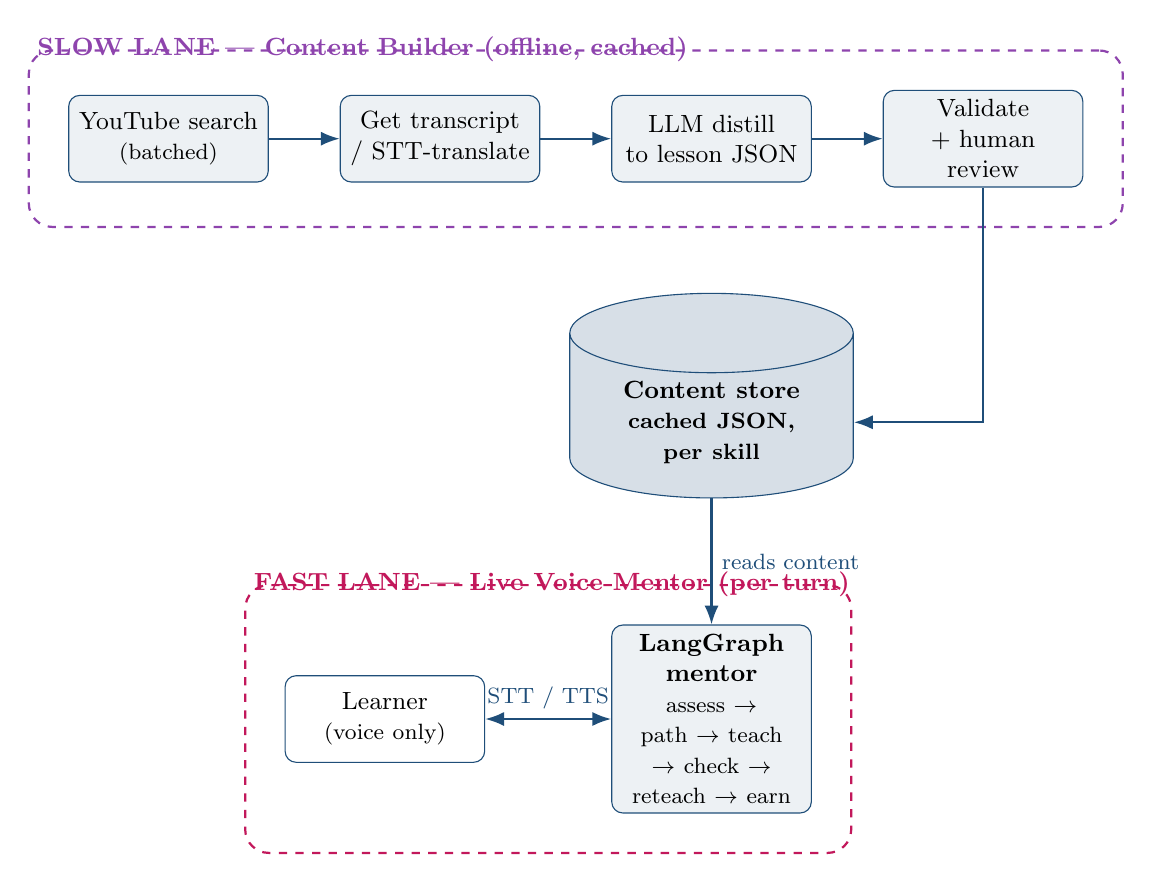
\begin{tikzpicture}[node distance=6mm and 9mm]

  % --- slow lane (top) ---
  \node[proc] (yt) {YouTube search \\ \footnotesize(batched)};
  \node[proc, right=of yt] (tr) {Get transcript \\ / STT-translate};
  \node[proc, right=of tr] (di) {LLM distill \\ to lesson JSON};
  \node[proc, right=of di] (va) {Validate \\ $+$ human review};

  % --- store (middle) ---
  \node[store, below=14mm of di] (store) {Content store \\ \footnotesize cached JSON, per skill};

  % --- fast lane (bottom) ---
  \node[proc, below=16mm of store] (mentor)
       {\textbf{LangGraph mentor} \\ \footnotesize assess $\to$ path $\to$ teach $\to$ check $\to$ reteach $\to$ earn};
  \node[io, left=16mm of mentor] (learner) {Learner \\ \footnotesize(voice only)};

  % --- arrows ---
  \draw[ar] (yt) -- (tr);
  \draw[ar] (tr) -- (di);
  \draw[ar] (di) -- (va);
  \draw[ar] (va.south) |- (store.east);
  \draw[ar] (store) -- node[right, font=\footnotesize, brand]{reads content} (mentor);
  \draw[arb] (learner) -- node[above, font=\footnotesize, brand]{STT / TTS} (mentor);

  % --- lane grouping boxes ---
  \begin{scope}[on background layer]
    \node[lane, slow, fit=(yt)(va)] (slowbox) {};
    \node[lane, fast, fit=(learner)(mentor)] (fastbox) {};
  \end{scope}
  \node[slow, font=\small\bfseries, anchor=west] at (slowbox.north west) {SLOW LANE --- Content Builder (offline, cached)};
  \node[fast, font=\small\bfseries, anchor=west] at (fastbox.north west) {FAST LANE --- Live Voice Mentor (per turn)};

\end{tikzpicture}
\end{center}

\noindent What is ``on the go'' is the \emph{assessment, path selection, narration, and visuals}.
The raw sourcing (video $+$ transcript) is pre-built and cached. A skill nobody has asked for before
triggers a background build --- \emph{``let me put that together for you''} --- then it is instant for
everyone after. Generated content and hand-authored content share one JSON shape, so they are
interchangeable to the engine.

% =========================================================================
\section{The slow lane: Content Builder}

Turns a \emph{skill or concept} into reusable, grounded teaching material, and never blocks a
conversation. Runs as a background job, or lazily on first request for a new skill, then caches.

\vspace{3mm}
\begin{center}
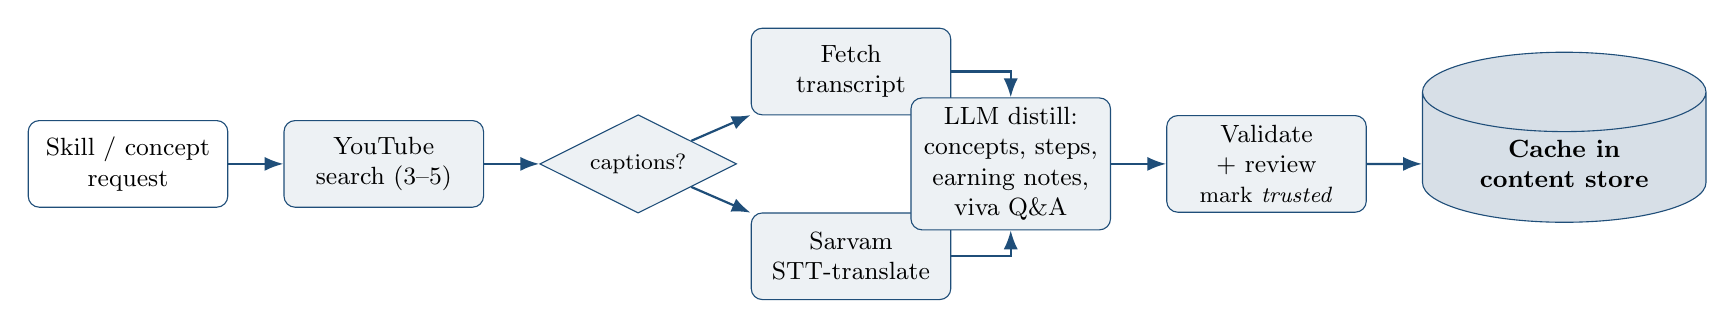
\begin{tikzpicture}[node distance=5mm and 7mm]
  \node[io] (req) {Skill / concept \\ request};
  \node[proc, right=of req] (search) {YouTube \\ search (3--5)};
  \node[dec, right=of search] (cap) {captions?};
  \node[proc, above right=3mm and 8mm of cap] (yes) {Fetch \\ transcript};
  \node[proc, below right=3mm and 8mm of cap] (no) {Sarvam \\ STT-translate};
  \node[proc, right=22mm of cap] (distill) {LLM distill: \\ concepts, steps, \\ earning notes, \\ viva Q\&A};
  \node[proc, right=of distill] (val) {Validate \\ $+$ review \\ \footnotesize mark \emph{trusted}};
  \node[store, right=of val] (cache) {Cache in \\ content store};

  \draw[ar] (req) -- (search);
  \draw[ar] (search) -- (cap);
  \draw[ar] (cap) -- (yes);
  \draw[ar] (cap) -- (no);
  \draw[ar] (yes) -| (distill);
  \draw[ar] (no)  -| (distill);
  \draw[ar] (distill) -- (val);
  \draw[ar] (val) -- (cache);
\end{tikzpicture}
\end{center}

\noindent The output is exactly the curriculum / rubric / visual-aid shape the existing teach engine
already reads. Each cached skill carries provenance (\code{source\_video\_ids}) and a \code{trusted}
flag. \textbf{Key constraint driving this design:} YouTube \code{search.list} is capped at roughly
100 searches/day (\S6), so searches are \emph{batched and cached}, never issued live per turn.

% =========================================================================
\section{The fast lane: learner journey}

Everything the learner experiences. Reads from the cache; generates only \emph{sequencing and
narration} live. Assessment is the differentiator: a woman who already sews never sits through
``this is a needle.''

\vspace{3mm}
\begin{center}
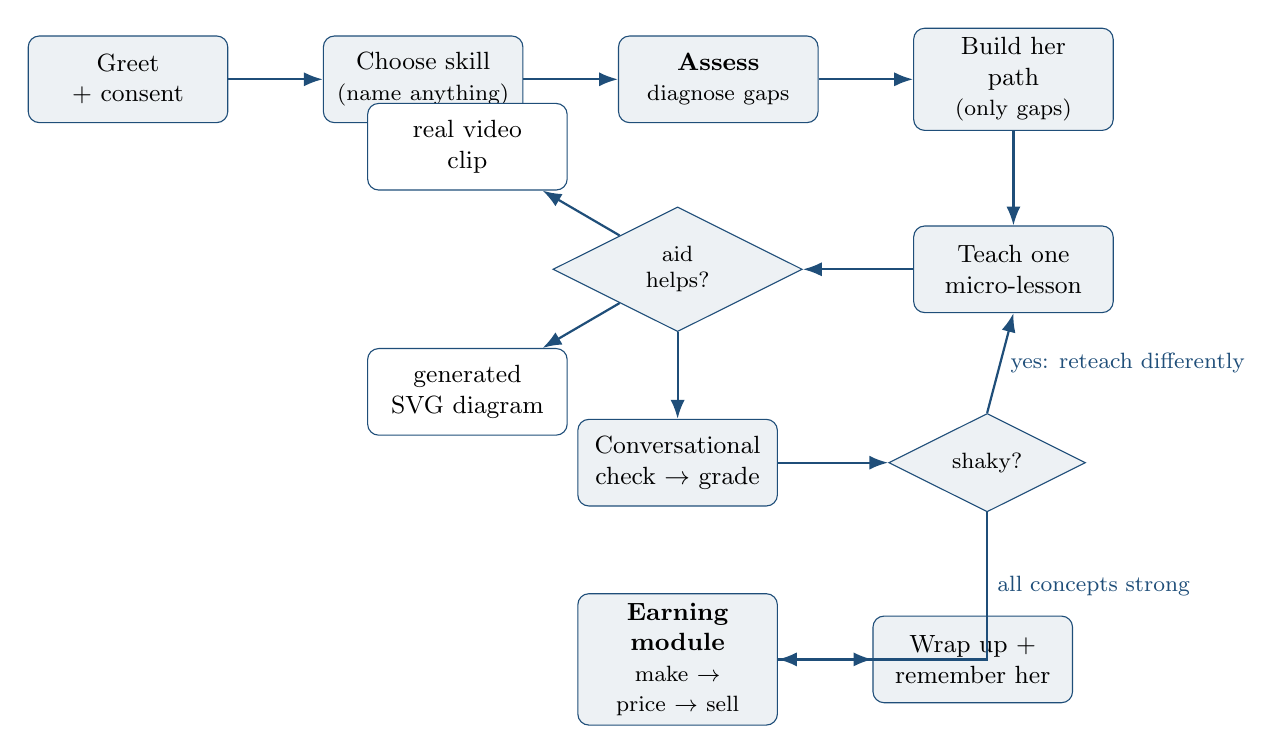
\begin{tikzpicture}[node distance=7mm and 12mm]
  \node[proc] (greet) {Greet \\ $+$ consent};
  \node[proc, right=of greet] (choose) {Choose skill \\ \footnotesize(name anything)};
  \node[proc, right=of choose] (assess) {\textbf{Assess} \\ \footnotesize diagnose gaps};
  \node[proc, right=of assess] (path) {Build her \\ path \\ \footnotesize(only gaps)};

  \node[proc, below=12mm of path] (teach) {Teach one \\ micro-lesson};
  \node[dec, left=14mm of teach] (aid) {aid \\ helps?};
  \node[io, above left=6mm and 6mm of aid] (video) {real video \\ clip};
  \node[io, below left=6mm and 6mm of aid] (svg) {generated \\ SVG diagram};
  \node[proc, below=11mm of aid] (check) {Conversational \\ check $\to$ grade};
  \node[dec, right=14mm of check] (shaky) {shaky?};

  \node[proc, below=11mm of check] (earn) {\textbf{Earning module} \\ \footnotesize make $\to$ price $\to$ sell};
  \node[proc, right=of earn] (wrap) {Wrap up $+$ \\ remember her};

  % top flow
  \draw[ar] (greet) -- (choose);
  \draw[ar] (choose) -- (assess);
  \draw[ar] (assess) -- (path);
  \draw[ar] (path) -- (teach);
  % teach -> aid -> back to teach (aids feed narration)
  \draw[ar] (teach) -- (aid);
  \draw[ar] (aid) -- (video);
  \draw[ar] (aid) -- (svg);
  \draw[ar] (aid) -- (check);
  % check -> shaky decision
  \draw[ar] (check) -- (shaky);
  % shaky yes -> reteach (loop back up to teach)
  \draw[ar] (shaky.north) -- node[right, font=\footnotesize, brand]{yes: reteach differently} (teach.south);
  % shaky no -> earn
  \draw[ar] (shaky.south) |- node[pos=0.25, right, font=\footnotesize, brand]{all concepts strong} (earn.east);
  \draw[ar] (earn) -- (wrap);
\end{tikzpicture}
\end{center}

% =========================================================================
\section{Content model (generalized --- no skill in code)}

The same three files as the original spec, now \emph{populated by the builder} rather than
hand-authored per trade:

\begin{itemize}
  \item \code{content/store/<skill>/curriculum.json} --- concepts $+$ ordered micro-steps $+$
  teaching notes $+$ \textbf{earning notes}, distilled from real tutorials; carries
  \code{source\_video\_ids} and a \code{trusted} flag.
  \item \code{content/store/<skill>/rubrics.json} --- viva questions $+$
  \code{sounds\_right}/\code{sounds\_confused} exemplars, drawn from the same transcripts.
  \item \code{content/store/<skill>/visual\_aids.json} --- vetted video clips (with timestamps) per
  concept; the reteach step may pick only from here, plus the live SVG-diagram generator as fallback.
\end{itemize}

\noindent The teach / viva / reteach engine reads this shape and \emph{never names a skill} --- so
adding candle-making, mehndi, or pickle-making is \emph{building and caching data}, not writing code.

% =========================================================================
\section{Feasibility findings (research, July 2026)}

\begin{center}
\renewcommand{\arraystretch}{1.25}
\begin{tabular}{p{3.4cm} p{1.7cm} p{7.2cm}}
\toprule
\textbf{Piece} & \textbf{Verdict} & \textbf{Detail / constraint} \\
\midrule
Get a video's transcript & works & \code{youtube-transcript-api} (free, no key) for captioned
videos; fallback Sarvam \textbf{STT-Translate} on the audio when captions are missing. Throttled
from cloud IPs $\rightarrow$ cache, do not refetch. \\
Understand Hindi/regional transcript & works & LLM comprehends; Sarvam Text Translation / Mayura
handles code-mixed Hinglish. \\
\textbf{Find} the right video live & \textbf{limited} & YouTube \code{search.list} $=100$ units,
capped $\approx100$ searches/day (own bucket since Jun 2026). $\rightarrow$ search offline/batched;
never live per turn. \emph{This is why the system is two-speed.} \\
Generate a visual live & use SVG & LLM $\to$ SVG/Mermaid diagrams are fast, cheap, consistent.
\emph{Avoid} diffusion/photo generation --- too detailed/inconsistent for low-literacy pictograms. \\
Assess-first $+$ adapt & founded & Matches current adaptive-learning research (cognitive diagnosis
$\to$ adaptive check $\to$ LLM feedback). The DB already has \code{concept\_mastery}. \\
Latency & watch & Turns already 5--8\,s. Keep the hot path to cached-read $+$ one cheap narration
call; all sourcing stays off-path. \\
\bottomrule
\end{tabular}
\end{center}

\noindent\footnotesize Sources: \url{https://www.sarvam.ai/models} ~\textbullet~
\url{https://pypi.org/project/youtube-transcript-api/} ~\textbullet~
\url{https://www.getphyllo.com/post/youtube-api-limits-how-to-calculate-api-usage-cost-and-fix-exceeded-api-quota}
~\textbullet~ \url{https://arxiv.org/pdf/2603.13695} ~\textbullet~
\url{https://smcleod.net/2024/10/generating-diagrams-with-with-ai-/-llms/} ~\textbullet~
\url{https://arxiv.org/pdf/2510.22559}
\normalsize

% =========================================================================
\section{What this reuses vs. changes}

\begin{center}
\renewcommand{\arraystretch}{1.2}
\begin{tabular}{p{5.3cm} p{7.4cm}}
\toprule
\textbf{Keep (T01--T14 plumbing)} & \textbf{Change / add} \\
\midrule
Repo, config, STT/TTS services, \code{/api/turn} pipeline, DB $+$ \code{concept\_mastery} $+$
persistence, UI command protocol, push-to-talk frontend, LangGraph skeleton, greet onboarding. &
\textbf{\code{assess}} becomes a real diagnostic (per-concept knowledge estimate, not a formality);
\textbf{Content Builder} (new); \textbf{SVG visual generator} (new, no-video fallback);
\code{teach}/\code{viva}/\code{reteach} read the cached store for \emph{any} skill; \textbf{earning
module} closes every skill; T15--T17 become ``seed \& review the starter library.'' \\
\bottomrule
\end{tabular}
\end{center}

% =========================================================================
\section{Open decisions}

\begin{enumerate}
  \item \textbf{New-skill latency:} build live in-session ($\approx$30--60\,s, magical) or in the
  background (safer, offer a seeded skill meanwhile)?
  \item \textbf{Reasoning stack:} keep OpenAI, or move to Sarvam's Chat LLM for a fully-sovereign
  Indic stack (better code-mixed handling, one vendor)?
  \item \textbf{Seed library size:} how many skills pre-built \& human-reviewed for the demo
  (recommend 3--4 deep, e.g. tailoring $+$ mehndi $+$ pickle-making), proving ``any skill'' live on
  one un-seeded example?
  \item \textbf{Review gate:} auto-trust builder output after validation, or require human sign-off
  before a generated skill is taught?
  \item \textbf{Visuals:} confirm they are \emph{optional aids only} (a screen may be absent) vs. an
  always-present supporting screen.
\end{enumerate}

\end{document}
